
\section{Experiment Details}\label{sec:appendix-experiment-details}

\subsection{Evaluated Models}
We provide the details of the baselines compared against \ours on the multimodal benchmark \mmebv (\autoref{tab:main_results}) and the text benchmark \beir (\autoref{tab:beir}) in~\autoref{appendix-model-configuration}.


\begin{table*}[htbp]
\centering
\small
%\renewcommand{\arraystretch}{1.1}
\resizebox{0.90\textwidth}{!}{%
\begin{tabular}{llcll}
\toprule[.1em]
\textbf{Model} & \textbf{Release} & \textbf{Retrieval} & \textbf{Backbone} & \textbf{\#Params} \\
\midrule
\multicolumn{5}{c}{\emph{\textbf{Baselines}}} \\
\midrule
Qwen3-VL-Embedding-8B  & 2026-01 & Dense  & Qwen3-VL-8B   & 8B   \\
Qwen3-VL-Embedding-2B  & 2026-01 & Dense  & Qwen3-VL-2B   & 2B   \\
RzenEmbed-V2-7B        & 2025-10 & Dense  & Qwen2-VL-7B   & 7B   \\
Embed-RL-4B            & 2026-02 & Dense  & Qwen3-VL-4B   & 4B   \\
Embed-RL-2B            & 2026-02 & Dense  & Qwen3-VL-2B   & 2B   \\
Ops-MM-Embed-7B        & 2025-07 & Dense  & Qwen2-VL-7B   & 7B   \\
Ops-MM-Embed-2B        & 2025-07 & Dense  & Qwen2-VL-2B   & 2B   \\
UniME-7B               & 2025-10 & Dense  & Qwen2-VL-7B   & 7B   \\
UniME-2B               & 2025-10 & Dense  & Qwen2-VL-2B   & 2B   \\
GME-7B                 & 2024-12 & Dense  & Qwen2-VL-7B   & 7B   \\
VLM2Vec-V2-2.0B        & 2025-05 & Dense  & Qwen2-VL-2B   & 2B   \\
SPLADE-v3              & 2024-03 & Sparse & BERT    & 110M \\
Echo-Mistral-SPLADE    & 2024-08 & Sparse & Mistral-7B    & 7B   \\
\midrule
\multicolumn{5}{c}{\emph{\textbf{Our model}}} \\
\midrule
\ours-2B               & 2026-08 & Dense \& Sparse & Qwen3.5-2B & 2B \\
\ours-4B               & 2026-08 & Dense \& Sparse & Qwen3.5-4B & 4B \\
\ours-9B               & 2026-08 & Dense \& Sparse & Qwen3.5-9B & 9B \\
\bottomrule
\end{tabular}
}
\caption{Details of the baselines compared against \ours. Multimodal models are evaluated on \mmebv; text-only models are evaluated on the nine \beir datasets reported in~\autoref{tab:beir}. \ours produces both dense and sparse embeddings from a single checkpoint.}
\label{appendix-model-configuration}
\end{table*}

\subsection{Evaluation Settings}

\paragraph{Metrics.} For MMEB-v2~\citep{vlm2vecv2}, we use its evaluation metrics for different datasets. For BEIR, we use nDCG@10 as the evaluation metric.

\paragraph{Score Calculation.} Unless otherwise noted, dense scores are cosine similarities of the EOS-token hidden states (\ie the last content token preceding the special tokens, as defined in~\S\ref{sec:method}), and sparse scores are inner products over the partitioned vocabulary representation defined in~\S\ref{sec:method}. 
 
\subsection{Details of Ablation Study}\label{sec:appendix-ablation-study}

\paragraph{Effectiveness.} We further detail the hybrid scoring used in~\S\ref{sec:effectiveness}. Given a query $q$ and a candidate $d$, the hybrid score linearly combines the dense cosine similarity $s_{\text{dense}}(q,d)$ and the sparse inner product $s_{\text{sparse}}(q,d)$ as
\begin{equation}
s_{\text{hybrid}}(q, d) = \alpha\, s_{\text{dense}}(q, d) + \beta\, s_{\text{sparse}}(q, d).
\end{equation}
Because $s_{\text{dense}}$ and $s_{\text{sparse}}$ lie on very different scales, dense cosine similarities are bounded in $[-1, 1]$ while sparse inner products can take much larger magnitudes. We fix $\alpha = 1.0$ and tune $\beta$ per modality on a held-out split. We use $\beta = 5\mathrm{e}{-8}$ for Text, $\beta = 5\mathrm{e}{-4}$ for Image, $\beta = 1\mathrm{e}{-4}$ for Video, and $\beta = 7\mathrm{e}{-4}$ for VisDoc. The optimum for plain text is several orders of magnitude smaller because raw sparse inner products grow rapidly with the number of activated tokens, whereas the heavier multimodal inputs yield much sparser activation patterns and therefore admit relatively larger $\beta$ values.


\paragraph{Efficiency.}
The sparse representations of \ours integrate natively with inverted indices, opening the door to large-scale lexical retrieval. To quantify this, we benchmark the offline retrieval mode of BrowseComp-Plus, comparing a Faiss-based dense index against a Lucene-backed sparse inverted index.
\autoref{fig:search-efficiency-comparison} illustrates the latency--accuracy trade-off of our sparse mode: by capping the maximum number of activated tokens per query ($K_{\mathrm{prune}}$), practitioners can flexibly trade search latency for retrieval quality (NDCG@5) to match deployment constraints. While dense search yields slightly higher absolute performance at this corpus size, we expect inverted-index retrieval to become increasingly favorable as the corpus grows; a systematic multi-scale evaluation is left to future work. 
\begin{figure}[htbp]
\centering
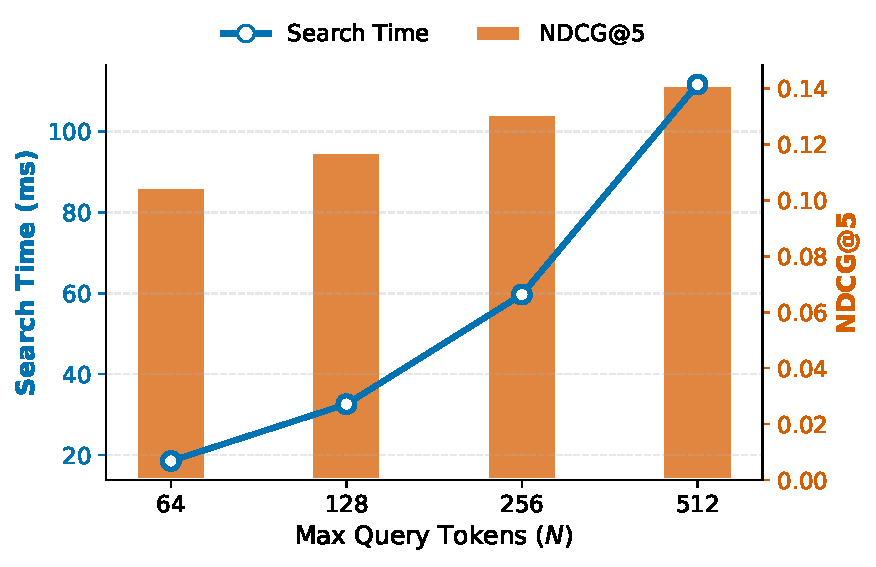
\includegraphics[width=0.6\linewidth]{resources/sparse_efficiency_comparison.pdf}
\caption{Search efficiency--effectiveness trade-off between dense retrieval and sparse inverted-index retrieval.}
\label{fig:search-efficiency-comparison}
\end{figure}

\subsection{Extra Experiment Results}

To provide a more reliable test of our hyperparameter settings, we report the MMEB-v2 results of models trained with random seed 42. These trends are broadly consistent with the main-paper settings: 
(1) joint dense-sparse training preserves dense performance while producing a competitive sparse branch ~\autoref{tab:ablation_mode}. 
(2) using too many special tokens hurts sparse retrieval ~\autoref{tab:ablation_nes}. 
(3) a higher sparse-training temperature is beneficial ~\autoref{tab:ablation_temperature}. 

\begin{table*}[htbp]
\centering
\renewcommand{\arraystretch}{1.1}
\setlength{\tabcolsep}{2.6pt}
\resizebox{\textwidth}{!}{
\begin{tabular}{l ccccc ccccc ccccc c}
\toprule
\multirow{2}{*}{\textbf{Mode}}
& \multicolumn{5}{c}{\textbf{Image}}
& \multicolumn{5}{c}{\textbf{Video}}
& \multicolumn{5}{c}{\textbf{VisDoc}}
& \multirow{2}{*}{\textbf{All}}\\
\cmidrule(lr){2-6} \cmidrule(lr){7-11} \cmidrule(lr){12-16}
& \textbf{CLS} & \textbf{QA} & \textbf{RET} & \textbf{GD} & \textbf{Avg.}
& \textbf{CLS} & \textbf{QA} & \textbf{RET} & \textbf{MRET} & \textbf{Avg.}
& \textbf{VDRv1} & \textbf{VDRv2} & \textbf{VR} & \textbf{OOD} & \textbf{Avg.} & \\
\midrule
\textbf{\# of Datasets} & 10 & 10 & 12 & 4 & 36 & 5 & 5 & 5 & 3 & 18 & 10 & 4 & 6 & 4 & 24 & 78 \\
\midrule
Dense-only & 55.3 & 65.4 & 65.3 & 83.5 & 64.6 & 56.3 & 52.2 & 44.8 & 48.3 & 50.6 & 81.6 & 61.7 & 82.9 & 66.8 & 76.1 & 64.9 \\
Sparse-only & 54.1 & 63.6 & 64.2 & 79.8 & 63.0 & 54.1 & 52.6 & 43.6 & 45.6 & 49.3 & 79.9 & 58.5 & 82.5 & 64.9 & 74.5 & 63.4 \\
UEmbed-2B (dense) & 55.5 & 65.3 & 65.1 & 83.3 & 64.5 & 58.3 & 46.9 & 45.6 & 47.5 & 49.8 & 81.6 & 59.5 & 83.1 & 66.7 & 75.8 & 64.6 \\
UEmbed-2B (sparse) & 54.7 & 63.1 & 64.8 & 81.8 & 63.4 & 56.0 & 46.3 & 44.4 & 45.7 & 48.4 & 79.9 & 59.3 & 82.0 & 65.9 & 74.7 & 63.4 \\
\bottomrule
\end{tabular}
}
\caption{MMEB-v2 performance comparison across representation modes.}
\label{tab:ablation_mode}
\end{table*}


\begin{table*}[htbp]
\centering
\renewcommand{\arraystretch}{1.1}
\setlength{\tabcolsep}{2.6pt}
\resizebox{\textwidth}{!}{
\begin{tabular}{l ccccc ccccc ccccc c}
\toprule[.1em]
\multirow{2}{*}{\textbf{$N$}}
& \multicolumn{5}{c}{\textbf{Image}}
& \multicolumn{5}{c}{\textbf{Video}}
& \multicolumn{5}{c}{\textbf{VisDoc}}
& \multirow{2}{*}{\textbf{All}}\\
\cmidrule(lr){2-6} \cmidrule(lr){7-11} \cmidrule(lr){12-16}
& \textbf{CLS} & \textbf{QA} & \textbf{RET} & \textbf{GD} & \textbf{Avg.}
& \textbf{CLS} & \textbf{QA} & \textbf{RET} & \textbf{MRET} & \textbf{Avg.}
& \textbf{VDRv1} & \textbf{VDRv2} & \textbf{VR} & \textbf{OOD} & \textbf{Avg.} & \\
\midrule
\textbf{\# of Datasets} & 10 & 10 & 12 & 4 & 36 & 5 & 5 & 5 & 3 & 18 & 10 & 4 & 6 & 4 & 24 & 78 \\
\midrule
2 & 56.0 & 62.9 & 65.0 & 81.2 & 63.7 & 56.6 & 48.2 & 45.3 & 46.6 & 49.4 & 80.1 & 59.4 & 82.1 & 65.8 & 74.8 & 63.8 \\
4 & 55.0 & 62.7 & 64.9 & 80.4 & 63.3 & 57.0 & 47.3 & 45.7 & 44.5 & 49.1 & 80.2 & 60.3 & 82.0 & 65.7 & 74.9 & 63.6 \\
8 & 54.9 & 62.2 & 65.2 & 81.0 & 63.2 & 55.1 & 48.9 & 44.8 & 46.1 & 49.0 & 79.6 & 58.8 & 81.6 & 65.8 & 74.3 & 63.4 \\
16 & 54.7 & 63.1 & 64.8 & 81.8 & 63.4 & 56.0 & 46.3 & 44.4 & 45.7 & 48.4 & 79.9 & 59.3 & 82.0 & 65.9 & 74.7 & 63.4 \\
32 & 54.6 & 62.8 & 65.0 & 80.3 & 63.2 & 54.4 & 46.2 & 41.9 & 45.7 & 47.2 & 75.6 & 22.3 & 73.4 & 65.7 & 64.5 & 59.9 \\
\bottomrule[.1em]
\end{tabular}
}
\caption{MMEB-v2 performance under different numbers of special tokens ($N$).}
\label{tab:ablation_nes}
\end{table*}


\begin{table*}[htbp]
\centering
\renewcommand{\arraystretch}{1.1}
\setlength{\tabcolsep}{2.6pt}
\resizebox{\textwidth}{!}{
\begin{tabular}{l ccccc ccccc ccccc c}
\toprule[.1em]
\multirow{2}{*}{\textbf{Temperature}}
& \multicolumn{5}{c}{\textbf{Image}}
& \multicolumn{5}{c}{\textbf{Video}}
& \multicolumn{5}{c}{\textbf{VisDoc}}
& \multirow{2}{*}{\textbf{All}}\\
\cmidrule(lr){2-6} \cmidrule(lr){7-11} \cmidrule(lr){12-16}
& \textbf{CLS} & \textbf{QA} & \textbf{RET} & \textbf{GD} & \textbf{Avg.}
& \textbf{CLS} & \textbf{QA} & \textbf{RET} & \textbf{MRET} & \textbf{Avg.}
& \textbf{VDRv1} & \textbf{VDRv2} & \textbf{VR} & \textbf{OOD} & \textbf{Avg.} & \\
\midrule
\textbf{\# of Datasets} & 10 & 10 & 12 & 4 & 36 & 5 & 5 & 5 & 3 & 18 & 10 & 4 & 6 & 4 & 24 & 78 \\
\midrule
2 & 53.7 & 61.7 & 62.8 & 77.4 & 61.6 & 50.7 & 48.6 & 41.7 & 44.3 & 46.6 & 79.5 & 57.5 & 80.0 & 64.4 & 73.4 & 61.8 \\
4 & 52.9 & 60.4 & 63.2 & 78.0 & 61.2 & 50.4 & 49.0 & 42.4 & 44.1 & 46.7 & 79.1 & 56.5 & 80.3 & 64.7 & 73.2 & 61.6 \\
8 & 55.0 & 60.8 & 64.5 & 80.2 & 62.6 & 54.9 & 50.6 & 43.2 & 43.6 & 48.6 & 80.3 & 58.1 & 81.6 & 65.3 & 74.4 & 63.0 \\
16 & 54.0 & 62.2 & 64.3 & 80.8 & 62.7 & 55.7 & 53.0 & 43.0 & 44.8 & 49.6 & 80.1 & 57.7 & 82.2 & 65.4 & 74.4 & 63.3 \\
32 & 54.7 & 63.1 & 64.8 & 81.8 & 63.4 & 56.0 & 46.3 & 44.4 & 45.7 & 48.4 & 79.9 & 59.3 & 82.0 & 65.9 & 74.7 & 63.4 \\
64 & 54.8 & 63.4 & 64.7 & 81.8 & 63.5 & 54.6 & 50.5 & 44.5 & 49.3 & 49.8 & 80.4 & 58.9 & 82.1 & 64.9 & 74.7 & 63.8 \\
\bottomrule[.1em]
\end{tabular}
}
\caption{MMEB-v2 performance under different temperature values.}
\label{tab:ablation_temperature}
\end{table*}
